\documentclass[40pt,a4paper,UTF8]{ctexart}
\usepackage{amsmath}
\usepackage{graphicx}

\usepackage{float}

%代码显示的包
\usepackage{listings}
\usepackage{xcolor}

%注释用
\usepackage{comment}
%----------------------------------------------
%配置代码显示格式-掌握minted之前的替代品
%----------------------------------------------
\definecolor{codegreen}{rgb}{0,0.6,0}
\definecolor{codegray}{rgb}{0.5,0.5,0.5}
\definecolor{codepurple}{rgb}{0.58,0,0.82}
\definecolor{backcolour}{rgb}{0.95,0.95,0.92}

\lstdefinestyle{mystyle}{
	backgroundcolor=\color{backcolour},   
	commentstyle=\color{codegreen},
	keywordstyle=\color{magenta},
	numberstyle=\tiny\color{codegray},
	stringstyle=\color{codepurple},
	basicstyle=\ttfamily\footnotesize,
	breakatwhitespace=false,         
	breaklines=true,                 
	captionpos=b,                    
	keepspaces=true,                 
	numbers=left,                    
	numbersep=5pt,                  
	showspaces=false,                
	showstringspaces=false,
	showtabs=false,                  
	tabsize=2
}

\lstset{style=mystyle}




%-----------------------------------------------------------------------------------

\title{第一章作业}
\author{Student name: Francisrk}
\date{Due date: January 23th, 2022}

\begin{document}

\maketitle   %控制序列,能将在导言区中定义的标题、作者、日期按照预定的格式展现出来。

\section{第1题}
\paragraph{}
已阅。
\paragraph{}

\section{第2题}
\subsection{要求1}
\paragraph{}

“apt-get install”安装软件包分为4步:
\begin{enumerate}
\item 扫描本地存放的软件包更新列表(由“apt-get update”命令刷新更新列表,也就是/var/lib/apt/lists/),找到最新版本的软件包
\item 进行软件包依赖关系检查,找到支持该软件正常运行的所有软件包
\item 从软件源所指 的镜像站点中,下载相关软件包
\item 解压软件包,并自动完成应用程序的安装和配置。
\end{enumerate}


依赖的意思就是你调用某个别人写好的函数之前需要使用某个包或者调用某个包。Ubuntu上用与Debian一样的Deb软件管理工具,apt-get就是Ubuntu的Deb软件管理工具,即APT包管理工具。这个软件会从Ubuntu的软件源库里调用安装所需要安装的包,而且可以自动分析和解决依赖关系,并且将所依赖的软件都安装完成。Ubuntu如果想安装指定版本的软件,可以在安装时在安装包名后边指定所要安装的版本即可。

\paragraph{}

\subsection{要求2}
\paragraph{}
软件源一般指debian系操作系统的应用程序安装包仓库,其中存放大量的软件包,apt会从软件源中下载软件,在/ect/apt/soure.list中可以为apt配置软件源。
更换系统自带的软件源:
\begin{lstlisting}[language=bash, caption=更换软件源]
#STEP1:备份源列表
sudo cp /etc/apt/sources.list /etc/apt/sources.list.bak  	
#STEP2:打开sources.list文件
sudo gedit /etc/apt/sources.list  							
#STEP3:将文件中的http://mirrors.aliyun.com/ubuntu/ 统一替换为(以阿里云为例)http://mirrors.aliyun.com/ubuntu/  保存退出
#STEP4:更新并升级(更新过程询问是否下载包,输入“y”)
sudo apt-get update && sudo apt-get upgrade
\end{lstlisting}

\paragraph{}

\subsection{要求3}
\paragraph{}

其他安装方式:
\begin{enumerate}
\item 下载deb包来进行安装:
\begin{lstlisting}[language=bash, caption=使用deb包进行安装]
sudo dpkg -i *.deb
\end{lstlisting}
\item make方式安装:对于某些软件仓库没有的库或者安装包,或者下载过慢的这种情况,我们可以选择直接下载其源码,然后进行源码安装。通常分为四步:配置–>编译–>安装–>清除临时文件:
\begin{lstlisting}[language=bash, caption=使用make进行安装]
git clone https://....
cd XXX
make
sudo make install
make clean
\end{lstlisting}

\item pip安装,这种方式不是Ubuntu自带的安装方式,需要在特定环境下安装
\begin{lstlisting}[language=bash, caption=使用pip进行安装]
pip install XXX
\end{lstlisting}
\end{enumerate}

其他发行版本的软件管理工具如图1.1所示
\begin{figure}[H]
\centering
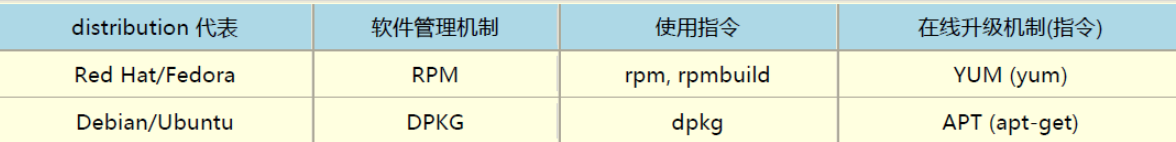
\includegraphics[width=4.8in]{ch1_1_1.png} {图1.1 其他发行版本的软件管理工具}
\end{figure}

\paragraph{}

\subsection{要求4}
\paragraph{}
环境变量PATH:指在操作系统中用来给系统和应用程序设置运行环境的一些参数,如临时文件夹位置和系统文件夹位置等,它包含了一个或多个应用程序将使用到的信息。

LD\_LIBRARY\_PATH:程序已经成功编译并且链接成功后,使用\\LD\_LIBRARY\_PATH来搜索目录,该变量中只有动态库有意义。


Idconfig的作用:ldconfig是一个动态链接库管理命令,为了让动态链接库为系统所共享,还需运行动态链接库的管理命令–ldconfig。Idconfig的用途,主要是在默认搜寻目录(/lib和/usr/lib)以及动态库配置文件/etc/ld.so.conf内所列的目录下,搜索出可共享的动态链接库(lib.so),进而创建出动态装入程序(ld.so)所需的连接和缓存文件.缓存文件默认为 /etc/ld.so.cache,此文件保存已排好序的动态链接库名字列表。

\paragraph{}

\subsection{要求5}
\paragraph{}
文件权限是指文件的访问控制,即那些用户和组群可以访问文件以及可以执行什么样的操作。默认情况下文件或目录的创建者即为该对象的属主。属主对文件或者目录有特别的操作权限。


访问权限规定三种不同类型的用户:
\\文件属主(Owner): 文件的所有者,称为属主。
\\同组用户(Group):文件属组的同组用户。
\\其它用户(Others):可以访问文件的其他用户。


访问权限的表示方法有三种,即三组九位字母表示法、三组九位二进制表示法和三位八进制表示法。其中用r表示读,用w表示写,用x表示可执行可查找,用-表示无权限。

文件权限的修改方法:修改文件权限的命令是chmod,执行该命令要求必须为文件属主或者是root用户才能使用。有两种修改方法,字母形式修改权限;数字形式修改权限。

\begin{lstlisting}[language=bash, caption=更改文件权限的两种方式]
#给a.sh添加可执行权限
sudo chmod +x a.sh   
#给a.sh的所有者赋予读写执行权限,所属群组和其他人均赋予读和执行权限
sudo chmod 755 a.sh 
\end{lstlisting}
\paragraph{}

\subsection{要求6}
\paragraph{}
Linux操作系统是多用户的分时操作系统,具有功能强大的用户管理机制,它将用户分为组,每个用户都属于某个组,每个用户都需要进行身份验证,同时用户只能在所属组所拥有的权限内工作,这样不仅方便管理,而且增加了系统的安全性。

用户:分为普通用户、管理员用户(root用户)和系统用户。普通用户在系统上的任务是进行普通的工作,root用户对系统具有绝对的控制权,但操作不当会对系统造成损毁。所以在进行简单任务是进行使用普通用户。

用户组:用户组是用户的容器,通过组,我们可以更加方便的归类、管理用户。用户能从用户组继承权限,一般分为普通用户组,系统用户组,私有用户组。当创建一个新用户时,若没有指定他所属于的组,系统就建立一个与该用户同名的私有组。当然此时该私有组中只包含这个用户自己。标准组可以容纳多个用户,若使用标准组,在创建一个新的用户时就应该指定他所属于的组。
\paragraph{}

\subsection{要求7}
\paragraph{}
gcc,g++,cmake,我的Ubuntu上默认是g++,它支持c++11标准。
\paragraph{}

\section{第3题}

\subsection{要求1} 
\paragraph{}
SLAM会在以下场景中用到:
\begin{enumerate}
\item 增强现实(AR):使用收集或者平板电脑观察家中的家具,在房间里摆放虚拟装饰品等。
\item 自动驾驶定位:在室内及遮挡严重的室外环境中,GPS定位精度低;高精度管道系统成本过高;基于无线信号的定位方案需要实现布置使用场景。而SLAM则可以直接使用相机或者激光雷达,在小场景范围内,勿需预先布置场景的情况下对车辆进行定位。
\item 无人机建图和定位:无人机在飞行的过程中需要知道哪里有障碍物,该怎么规避,怎么重新规划路线。
\item 智能家居定位和建图:如扫地机需要使用二维的激光SLAM定位并构建家里的地图,规划扫地路线。
\end{enumerate}

\paragraph{}


\subsection{要求2} 
\paragraph{}
定位:系统要明白自身的状态(即位置);
建图:系统也要了解外在的环境(即地图)
定位和见图是紧密耦合的,根据\cite{ref1}:
\\ Being precisely localized in an environment,a correct map is necessary, but in order to construct a good map it is necessary to be properly localized when elements are added to the map. 在一个环境中精确定位之后,一个正确的地图是必要的,但为了构建一个好的地图,当新的元素加到地图中时需要精准地定位。


\paragraph{}

\subsection{要求3} 
\paragraph{}
根据\cite{ref1},SLAM可分为两阶段:古典阶段和算法分析阶段:
\begin{enumerate}
\item 1986-2004 年,古典年代,这个阶段从 SLAM 的提出到建立完整的系统,引入了 SLAM概率论推导方法,包括基于扩展卡尔曼滤波、粒子滤波和最大似然估计,同时,面临效率和数据关联鲁棒性问题的挑战;
\item 2004-2015 年,算法分析年代,这一阶段有许多包括可观测性,收敛性和一致性的SLAM 基本特性研究,理解了稀疏特征在高效 SLAM 解决方案中的重要角色,并且开发了许多开源SLAM库。
\end{enumerate}
\paragraph{}

\subsection{要求4} 
\paragraph{}

  在2010年出现基于视觉SLAM的方法之后将SLAM分为前端和后端。


总的来说,SLAM本质上是对运动主体自身和周围环境空间不确定性的估计。前端根据状态估计理论,把定位和建图的不确定性表达出来,送给后端,后端采用滤波器或非线性优化,估计状态的均值何不确定性。


具体来说,前端全称叫做“前端视觉历程计”(VO),其任务是估算相邻图像间相机的运动,以及局部地图的样子,理论上来说,一方面,将相邻时刻的运动串起来,就构成了机器人的运动轨迹,从而解决了定位问题;另一方面,根据每个时刻的相机位置,计算出各像素对应的空间点的位置,就得到了地图。但是实际中,仅通过视觉历程计来估计轨迹会出现累计漂移,而为了解决漂移问题,需要引入后端优化和回环检测,其中,后端全称叫后端非线性优化,其接受不同是可视觉里程计的相机位姿以及回环检测的信息,对他们进行优化,得到全局一致的轨迹和地图。
\paragraph{}



\subsection{要求5} 
\paragraph{}
\begin{enumerate}
\item MonoSLAM,首个单目V-SLAM系统\cite{ref2}.
\item PTAM,首个基于关键帧BA的单目V-SLAM系统\cite{ref3}.
\item LSD-SLAM,单目直接法的代表系统\cite{ref4}.
\end{enumerate}



\paragraph{}

\section{第4题}

\subsection{要求1,2,3} 
\paragraph{}
工程组织如图4.1所示


\begin{figure}[H]
\centering

\includegraphics[width=4.8in]{ch1_4_1.png} {图4.1 工程组织图}
\end{figure}


编译出来sayhello置于main文件夹下,执行sayhello并输出,如图4.2所示
\begin{figure}[H]
\centering
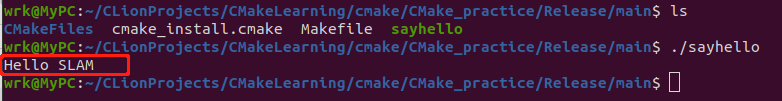
\includegraphics[width=4.8in]{ch1_4_2.png} {图4.2 sayhello输出}
\end{figure}

各部分代码如下:



\begin{lstlisting}[language=bash, caption=按照Release方式编译工程]
mkdir Release && cd Release
cmake -DCMAKE_BUILD_TYPE=Release .. 
\end{lstlisting}


\begin{lstlisting}[language=bash, caption=工程/CMakeLists.txt]
PROJECT(CMAKE_)
ADD_SUBDIRECTORY(include)
ADD_SUBDIRECTORY(src)
ADD_SUBDIRECTORY(main)
ADD_SUBDIRECTORY(cmake)
\end{lstlisting}


\begin{lstlisting}[language=bash, caption=include/CMakeLists.txt]
INSTALL(FILES hello.h DESTINATION include/hello)
\end{lstlisting}


\begin{lstlisting}[language=bash, caption=src/CMakeLists.txt]
FIND_PATH(myHeader hello.h)
INCLUDE_DIRECTORIES(../include)  #添加一个头文件搜索路径
SET(LIBHELLO_SRC hello.cpp)
ADD_LIBRARY(hello SHARED ${LIBHELLO_SRC})
ADD_LIBRARY(hello_static STATIC ${LIBHELLO_SRC})
SET_TARGET_PROPERTIES(hello_static PROPERTIES OUTPUT_NAME "hello")
GET_TARGET_PROPERTY(OUTPUT_VALUE hello_static OUTPUT_NAME)
MESSAGE(STATUS "this is the hello_static OUTPUT_NAME:"${OUTPUT_VALUE})
SET_TARGET_PROPERTIES(hello PROPERTIES VERSION 1.2 SOVERSION 1)
SET_TARGET_PROPERTIES(hello PROPERTIES CLEAN_DIRECT_OUTPUT 1)
SET_TARGET_PROPERTIES(hello_static PROPERTIES CLEAN_DIRECT_OUTPUT 1)
INSTALL(TARGETS hello hello_static LIBRARY DESTINATION lib ARCHIVE DESTINATION lib)
\end{lstlisting}


\begin{lstlisting}[language=bash, caption=main/CMakeLists.txt]
ADD_EXECUTABLE(sayhello useHello.cpp)
TARGET_LINK_LIBRARIES(sayhello hello)
INCLUDE_DIRECTORIES(../include)  #添加一个头文件搜索路径
\end{lstlisting}

\paragraph{}


\subsection{要求4} 
库的安装结果如图4.3所示:

\begin{figure}[H]
\centering
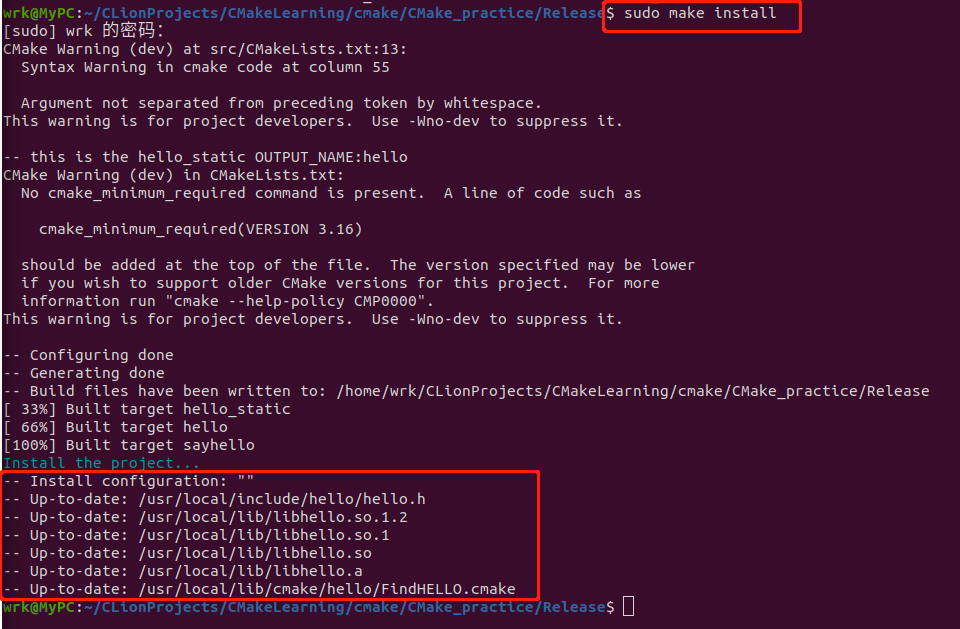
\includegraphics[width=4.8in]{ch1_4_3.png} {图4.3 hello库的安装结果}
\end{figure}

\subsection{要求5} 
\paragraph{}

hello库的FindHello.cmake文件用于寻找库,
\begin{lstlisting}[language=bash, caption=hello工程/cmake/FindHELLO.cmake]
FIND_PATH(HELLO_INCLUDE_DIR hello.h /usr/include/hello /usr/local/include/hello)
FIND_LIBRARY(HELLO_LIBRARY NAMES hello PATH /usr/lib   /usr/local/lib)
IF (HELLO_INCLUDE_DIR AND HELLO_LIBRARY)
SET(HELLO_FOUND TRUE)
ENDIF (HELLO_INCLUDE_DIR AND HELLO_LIBRARY)
IF (HELLO_FOUND)
IF (NOT HELLO_FIND_QUIETLY)
MESSAGE(STATUS "Found Hello: ${HELLO_LIBRARY}")
ENDIF (NOT HELLO_FIND_QUIETLY)
ELSE (HELLO_FOUND)
IF (HELLO_FIND_REQUIRED)
MESSAGE(FATAL_ERROR "Could not find hello library")
ENDIF (HELLO_FIND_REQUIRED)
ENDIF (HELLO_FOUND)
\end{lstlisting}

\begin{lstlisting}[language=bash, caption=hello工程/cmake/CMakeLists.txt]
INSTALL(FILES FindHELLO.cmake DESTINATION lib/cmake/hello)  #把FindHELLO.cmake安装到对应位置
\end{lstlisting}

建立工程Find如图4.4所示
\begin{figure}[H]
\centering
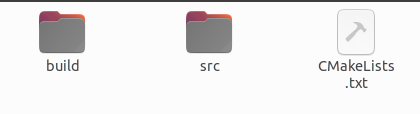
\includegraphics[width=4.8in]{ch1_4_4.png} {图4.4 测试工程Find的工程组织}
\end{figure}




\begin{lstlisting}[language=bash, caption=工程/CMakeLists.txt]
PROJECT(Find)
cmake_minimum_required(VERSION 3.16)
SET(HELLO_DIR /usr/local/lib)  #库文件位置
SET(CMAKE_MODULE_PATH /usr/local/lib/cmake/hello)  #FindHELLO.cmake位置
ADD_SUBDIRECTORY(src)
\end{lstlisting}


\begin{lstlisting}[language=bash, caption=src/CMakeLists.txt]
FIND_PACKAGE(HELLO)
IF(HELLO_FOUND)
	ADD_EXECUTABLE(helloexe main.cpp)
	INCLUDE_DIRECTORIES(${HELLO_INCLUDE_DIR})  #添加头文件搜索路径
	TARGET_LINK_LIBRARIES(helloexe ${HELLO_LIBRARY}) #链接
	
	MESSAGE(STATUS "The HELLO_INCLUDE_DIR is:"${HELLO_INCLUDE_DIR})
	MESSAGE(STATUS "The HELLO_LIBRARY is:"${HELLO_LIBRARY})	
ENDIF(HELLO_FOUND)
\end{lstlisting}

\begin{lstlisting}[language=C++, caption=src/CMakeLists.txt]
#include "hello.h"
int main()
{
	sayHello();
	return 0;
}
\end{lstlisting}

测试过程和结果如图4.5所示
\begin{figure}[H]
\centering
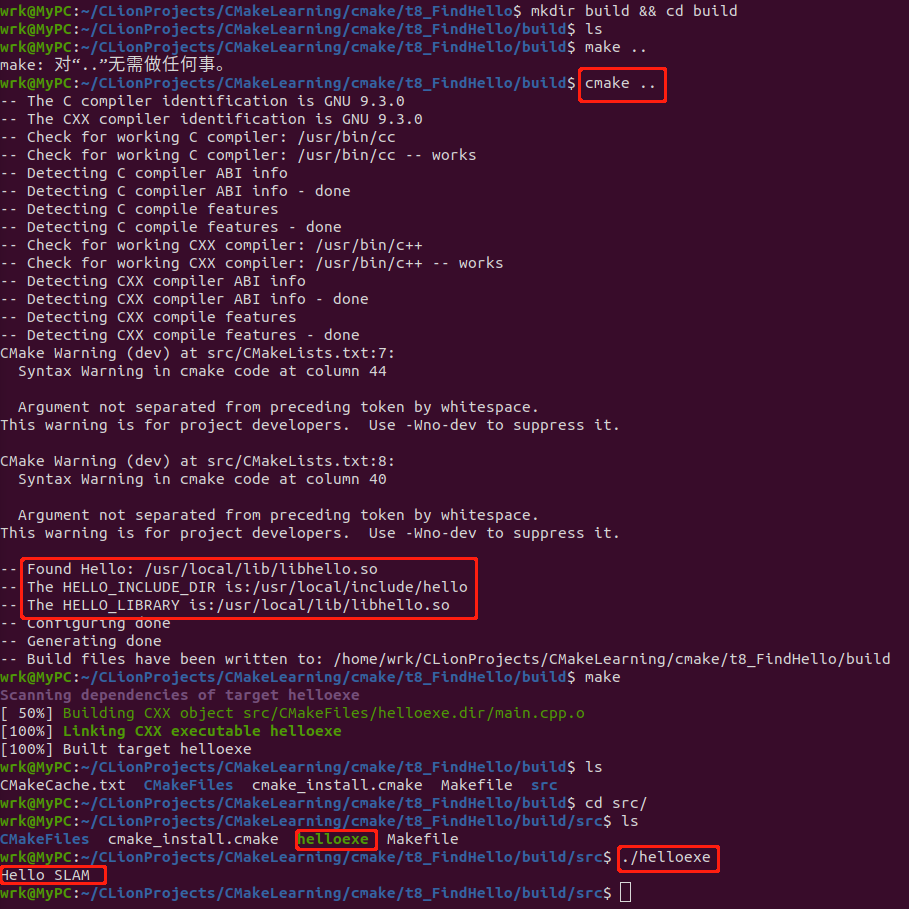
\includegraphics[width=4.8in]{ch1_4_5.png} {图4.5 测试过程和结果}
\end{figure}


\paragraph{}


\section{第5题}
\subsection{要求1} 
\paragraph{}

gflags安装
\begin{lstlisting}[language=bash, caption=gflags安装]
git clone https://github.com/gflags/gflags.git
cd gflags
mkdir build && cd build
cmake -DCMAKE_INSTALL_PREFIX=/usr/local -DBUILD_SHARED_LIBS=ON -DGFLAGS_NAMESPACE=gflags ../
make -j4
sudo make install
\end{lstlisting}

glog安装
\begin{lstlisting}[language=bash, caption=glog安装]
git clone https://github.com/google/glog
cd glog/
mkdir build && cd build
cmake ..
make -j4
sudo make install
\end{lstlisting}

gtest安装:
https://github.com/google/googletest/releases 下载release-1.8.1.tar.gz 
\begin{lstlisting}[language=bash, caption=gtest安装]
tar -xzvf googletest-release-1.8.1.tar.gz
cd googletest-release-1.8.1/
mkdir build && cd build
cmake ..
make
sudo make install
\end{lstlisting}
\paragraph{}

\subsection{要求2,3} 
\paragraph{}

改成glog打印,运用gflags传入打印次数print\_times为10次并输出,结果如图5.1所示

\begin{figure}[H]
\centering
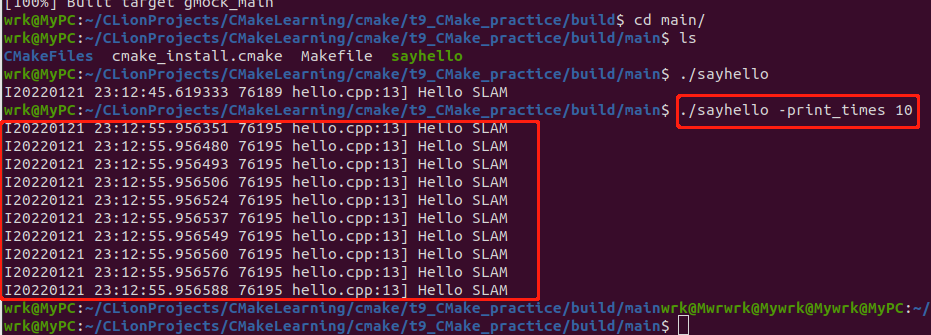
\includegraphics[width=4.8in]{ch1_5_1.png} {图5.1 glog打印,传入gflags参数测试结果}
\end{figure}


\begin{lstlisting}[language=bash, caption=工程/CMakeLists.txt]
PROJECT(CMAKE_)
ADD_SUBDIRECTORY(include)
ADD_SUBDIRECTORY(src)
ADD_SUBDIRECTORY(main)
ADD_SUBDIRECTORY(cmake)
ADD_SUBDIRECTORY(test)
\end{lstlisting}

\begin{lstlisting}[language=bash, caption=include/CMakeLists.txt]
FIND_PACKAGE(gflags REQUIRED)
INSTALL(FILES hello.h DESTINATION include/hello)
\end{lstlisting}

\begin{lstlisting}[language=C++, caption=include/hello.h]
#pragma once
#include <gflags/gflags.h>

DECLARE_int32(tmp);
void sayHello(); 
long my_fac(long n);
\end{lstlisting}

\begin{lstlisting}[language=bash, caption=src/CMakeLists.txt]
INCLUDE_DIRECTORIES(../include)  #添加一个头文件搜索路径

SET(LIBHELLO_SRC hello.cpp)
ADD_LIBRARY(hello SHARED ${LIBHELLO_SRC})
ADD_LIBRARY(hello_static STATIC ${LIBHELLO_SRC})
SET_TARGET_PROPERTIES(hello_static PROPERTIES OUTPUT_NAME "hello")
GET_TARGET_PROPERTY(OUTPUT_VALUE hello_static OUTPUT_NAME)
MESSAGE(STATUS "this is the hello_static OUTPUT_NAME:"${OUTPUT_VALUE})
SET_TARGET_PROPERTIES(hello PROPERTIES VERSION 1.2 SOVERSION 1)
SET_TARGET_PROPERTIES(hello PROPERTIES CLEAN_DIRECT_OUTPUT 1)
SET_TARGET_PROPERTIES(hello_static PROPERTIES CLEAN_DIRECT_OUTPUT 1)

FIND_PACKAGE(gflags REQUIRED)  #找到gflags包
FIND_PACKAGE(glog REQUIRED)    #找到glog包

INSTALL(TARGETS hello hello_static LIBRARY DESTINATION lib ARCHIVE DESTINATION lib)
\end{lstlisting}

\begin{lstlisting}[language=C++, caption=src/hello.cpp]
#include "hello.h"
#include <iostream>

#include <gflags/gflags.h>
#include <glog/logging.h>

DEFINE_int32(tmp, 100, "This is temp test value!");


void sayHello()
{
        FLAGS_logtostderr = 1;  //输出到控制台
        LOG(INFO) <<"Hello SLAM";
}

long my_fac(long n)
{
        if(n<1) return 1;
        else    return n*my_fac(n-1);
}
\end{lstlisting}

\begin{lstlisting}[language=bash, caption=main/CMakeLists.txt]
INCLUDE_DIRECTORIES(../include)  #添加一个头文件搜索路径
FIND_PACKAGE(gflags REQUIRED)  #找到gflags包
FIND_PACKAGE(glog REQUIRED)    #找到glog包
ADD_EXECUTABLE(sayhello useHello.cpp)
TARGET_LINK_LIBRARIES(sayhello hello gflags glog) 
\end{lstlisting}

\begin{lstlisting}[language=C++, caption=main/main.cpp]
#include <iostream>
#include "hello.h"
#include <gflags/gflags.h>
#include <glog/logging.h>

DEFINE_int32(print_times, 1, "The print times");  #定义打印次数gflags

int main( int argc, char** argv )
{
        gflags::ParseCommandLineFlags(&argc, &argv, true);  //用于接受命令行的flag参数并更新默认参数
        google::InitGoogleLogging("daqing");    //初始化一个log
        FLAGS_logtostderr = 1;  //输出到控制台
        for(int i=FLAGS_print_times; i>0;--i)
          sayHello();
        google::ShutdownGoogleLogging();    //不用log时进行释放
        return 0;
}
\end{lstlisting}

\paragraph{}

\subsection{要求4} 
\paragraph{}

在hello.cpp中写了一个阶乘的函数my\_fac(long n),放在test/main\_test中进行测试,结果如图5.2所示

\begin{figure}[H]
\centering
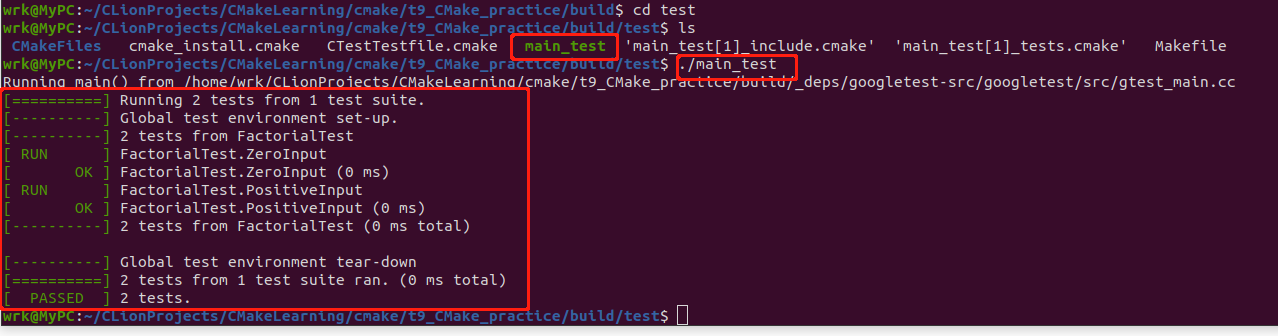
\includegraphics[width=4.8in]{ch1_5_2.png} {图5.2 gtest测试结果}
\end{figure}

\begin{lstlisting}[language=bash, caption=test/CMakeLists.txt]
INCLUDE_DIRECTORIES(../include)  #hello.h搜索路径
FIND_PACKAGE(gflags REQUIRED)  #找到gflags包
FIND_PACKAGE(glog REQUIRED)    #找到glog包

set(CMAKE_CXX_STANDARD 11)
include(FetchContent)  #载入模块
FetchContent_Declare(
  googletest
  URL https://github.com/google/googletest/archive/609281088cfefc76f9d0ce82e1ff6c30cc3591e5.zip)

set(gtest_force_shared_crt ON CACHE BOOL "" FORCE)
FetchContent_MakeAvailable(googletest)

enable_testing()
add_executable(  main_test  main_test.cpp)
target_link_libraries(main_test  gtest_main hello gflags glog)

#使CMake runner能够在二进制中找到测试,使用GoogleTest模块
include(GoogleTest)  
gtest_discover_tests(main_test) 
\end{lstlisting}

\begin{lstlisting}[language=C++, caption=test/main\_test.txt]
#include <gtest/gtest.h>
#include <gflags/gflags.h>
#include <glog/logging.h>
#include <hello.h>

TEST(FactorialTest, ZeroInput){
        EXPECT_EQ(my_fac(0), 1);}

TEST(FactorialTest, PositiveInput){
        EXPECT_EQ(my_fac(1), 1);
        EXPECT_EQ(my_fac(2), 2);
        EXPECT_EQ(my_fac(3), 6);}
\end{lstlisting}


整个工程树如图5.3所示
\begin{figure}[H]
\centering
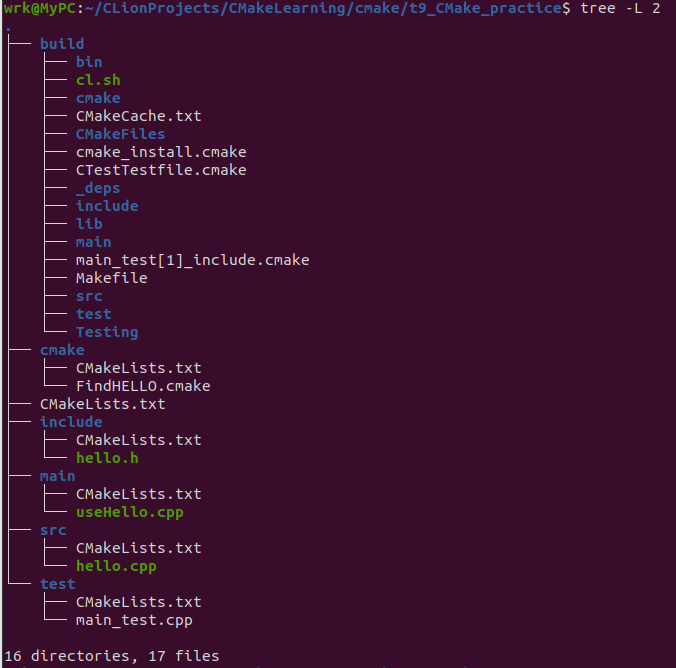
\includegraphics[width=4.8in]{ch1_5_3.png} {图5.3 整个工程树}
\end{figure}

\paragraph{}


%------------------------------------------------------------------------------
\section{第6题}
\subsection{要求1} 
\paragraph{}
下载ORB-SLAM2结果如图6.1所示
\begin{figure}[H]
\centering
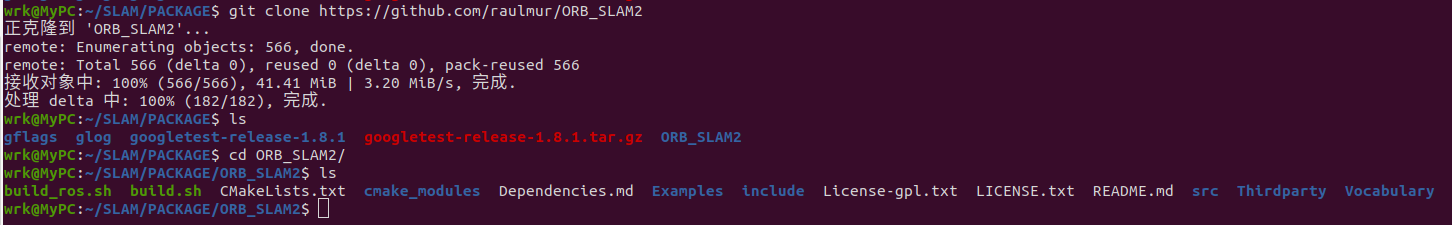
\includegraphics[width=4.8in]{ch1_6_1.png} {图6.1 下载ORB-SLAM2完成}
\end{figure}

\paragraph{}

\subsection{要求2} 
\paragraph{}
\begin{enumerate}
\item ORB-SLAM将在\${PROJECT\_SOURCE\_DIR}/lib文件夹下编译出19个动态库文件,在\${PROJECT\_SOURCE\_DIR}/Examples文件夹下的3个子文件夹分别编译出6个可执行文件rgbd\_tum,stereo\_kitti,stereo\_euroc,mono\_tum,mono\_kitti,mono\_euroc。
\item include中包含了ORB-SLAM2建立的库的头文件(20项);src中包含了ORB-SLAM2建立的库的源文件(19项);Exemples包含编译出的6个可执行文件,放在3个文件夹中,ROS文件夹下放的推测应该是在ROS系统下能运行的Demo。
\item 可执行文件链接了5个库:OpenCV,EIGEN3,Pangolin,libDBoW2,libg2o。
\end{enumerate}

\paragraph{}

%------------------------------------------------------------------------------
\section{第7题}
\subsection{要求1} 
\paragraph{}
编译成功,如图7.1所示
下载ORB-SLAM2结果如图7.1所示
\begin{figure}[H]
\centering
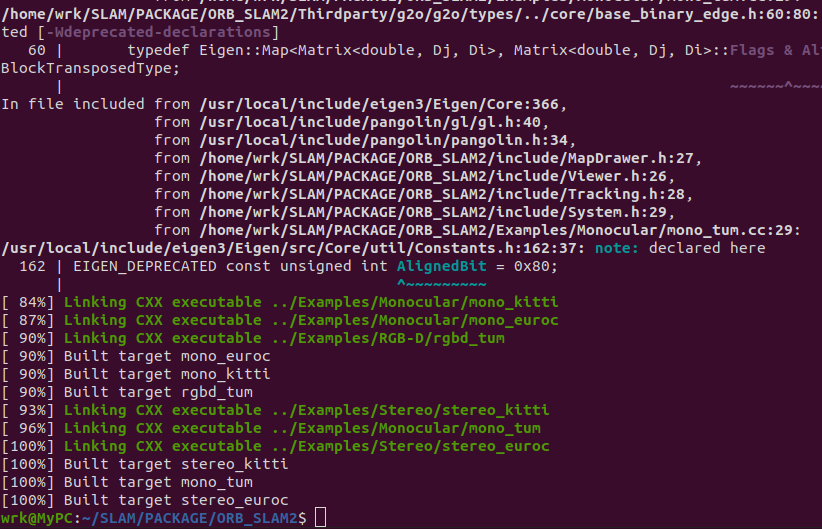
\includegraphics[width=4.8in]{ch1_7_1.png} {图7.1 编译ORB-SLAM2成功}
\end{figure}

\paragraph{}

\subsection{要求2} 
\paragraph{}
在工程的CMakeLists.txt下添加这几句话:

\begin{lstlisting}[language=bash, caption=修改的工程/CMakeLists.txt]
set(CMAKE_RUNTIME_OUTPUT_DIRECTORY ${PROJECT_SOURCE_DIR}/Examples/Myvideo)
#给的视频
#add_executable(myvideo	
#Examples/Myvideo/myvideo.cpp)
#target_link_libraries(myvideo ${PROJECT_NAME})	
#自己的相机
add_executable(myslam	
Examples/Myvideo/myslam.cpp)
target_link_libraries(myslam ${PROJECT_NAME})
\end{lstlisting}

对应的文件路径修改

\begin{lstlisting}[language=c++, caption=MyVideo/myslam.cpp部分修改]
string parameterFile = "./myvideo.yaml";
string vocFile = "../../Vocabulary/ORBvoc.txt";
\end{lstlisting}

\paragraph{}

\subsection{要求3} 
\paragraph{}
运行自己电脑的摄像头结果如图7.2所示
\begin{figure}[H]
\centering
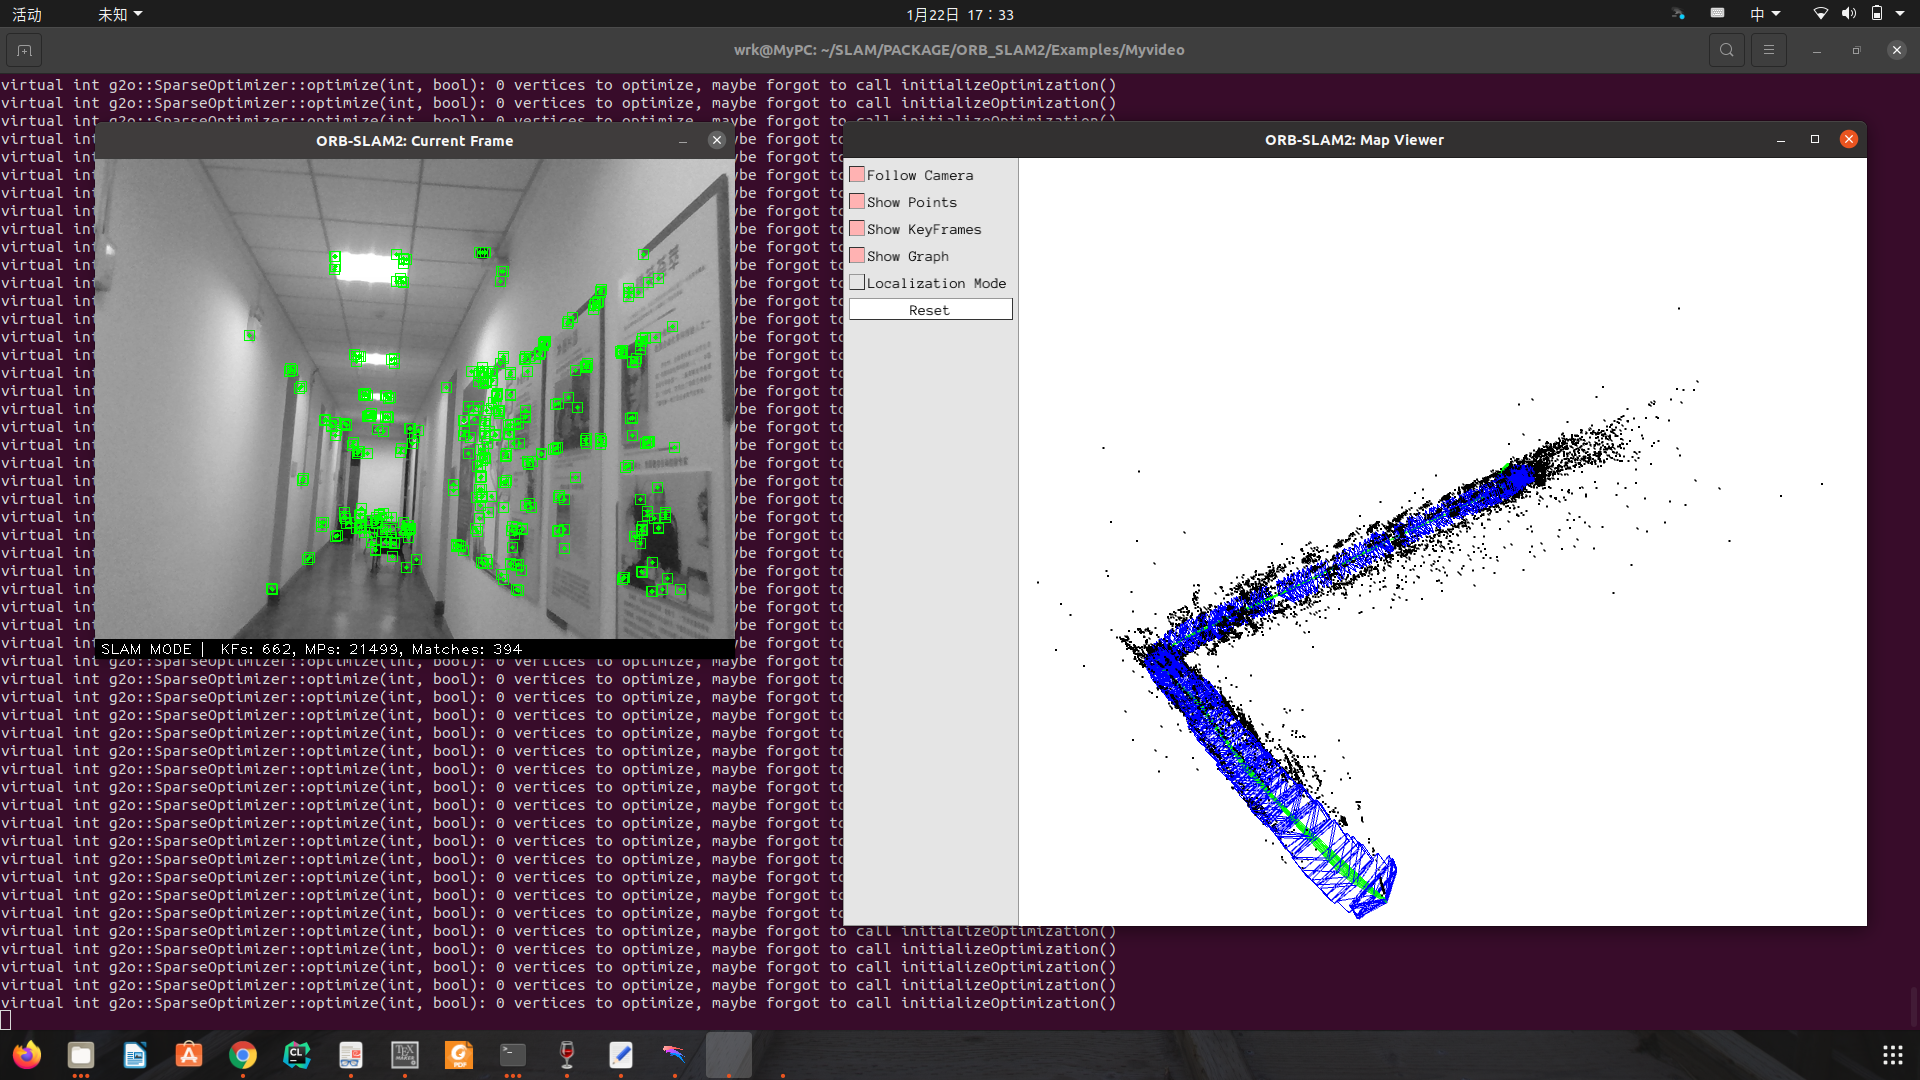
\includegraphics[width=4.8in]{ch1_7_2.png} {图7.2 电脑摄像头运行ORB-SLAM2}
\end{figure}

运行给的视频结果如图7.3所示
\begin{figure}[H]
\centering
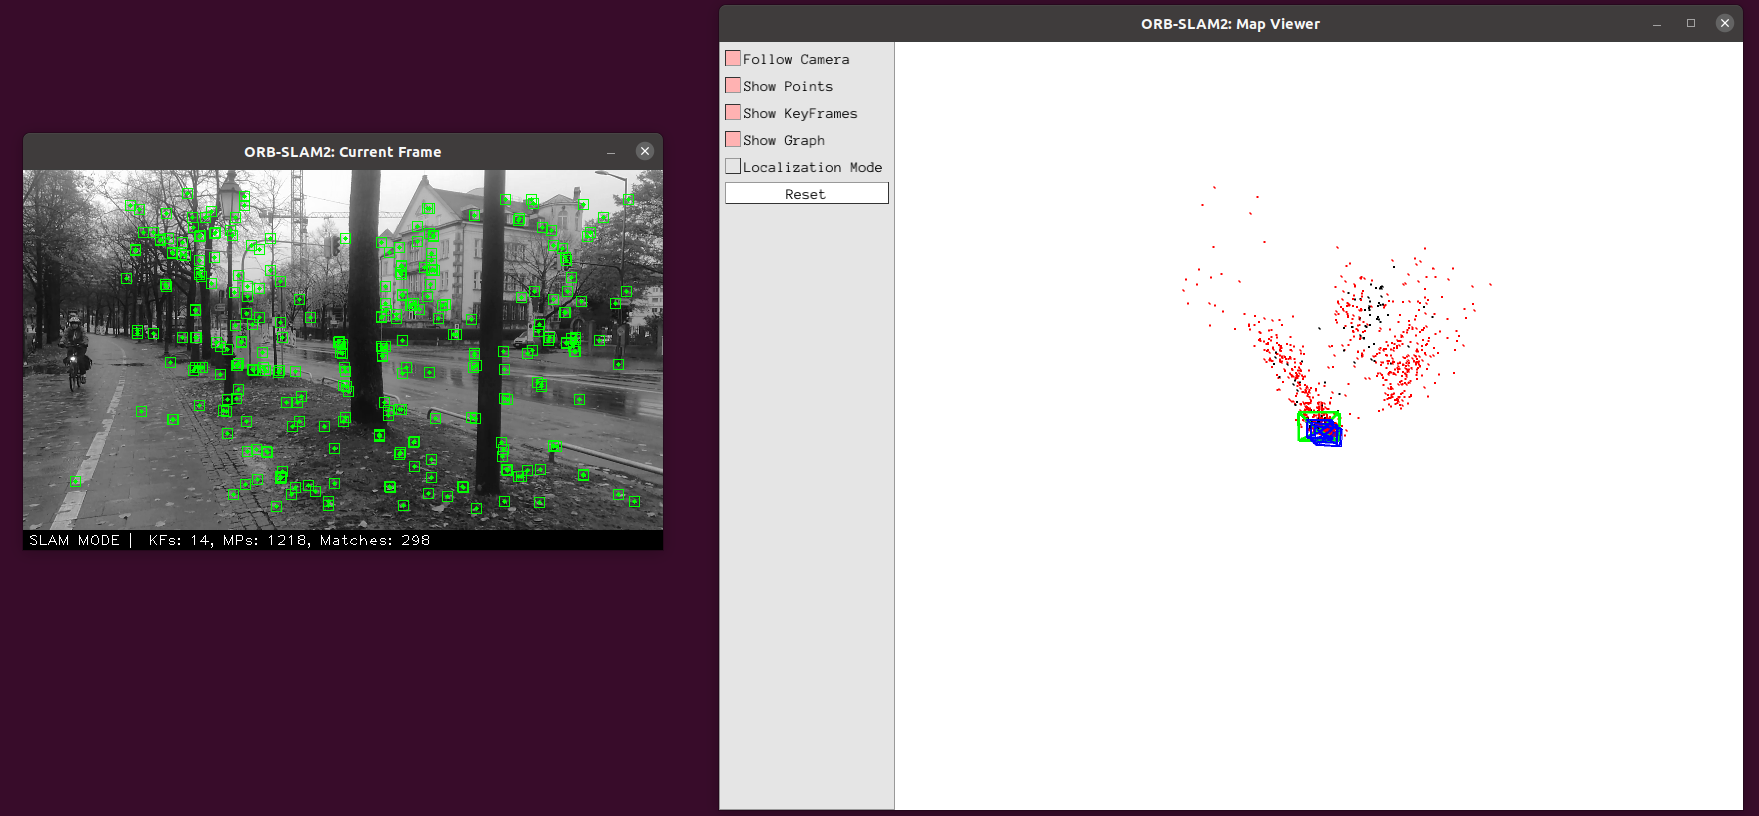
\includegraphics[width=4.8in]{ch1_7_3.png} {图7.3 给的视频运行ORB-SLAM2}
\end{figure}


运行体会:我尝试在实验楼构建一个带有回环的地图,但是走到白色的墙比较多,特征点比较少的地方就丢掉了tracking,怎么都过不去,比如如果进了隧道,什么都看不见,但是还是得能构建的出来地图,比如保持当前的方向,出来之后再进行补偿之类的,我想这应该是ORB-SLAM2一个缺陷吧,总之,第一次跑出SLAM还是挺开心的。


\paragraph{}

\begin{thebibliography}{99}  
\bibitem{ref1}J. Fuentes-Pacheco, J. Ruiz-Ascencio, and J. M. Rendón-Mancha, “Visual simultaneous localization and mapping: a survey,” Artificial Intelligence Review, vol. 43, no. 1, pp. 55–81, 2015.

\bibitem{ref2}Davison A J, Reid I D, Molton N D, et al. MonoSLAM: real- time single camera SLAM[J]. IEEE Transactions on Pattern Analysis and Machine Intelligence, 2007, 29(6):1052-1067

\bibitem{ref3}Klein, Georg S. W. and David William Murray. “Parallel Tracking and Mapping for Small AR Workspaces.” 2007 6th IEEE and ACM International Symposium on Mixed and Augmented Reality (2007): 225-234.

\bibitem{ref4}Engel, Jakob et al. “LSD-SLAM: Large-Scale Direct Monocular SLAM.” ECCV (2014).
\end{thebibliography}


\end{document}